\subsection{Result-Dashboard}
\label{ssec:konzept:client:dashboard}

Das Dashboard stellt die Kernkomponente dieser Anwendung für Nutzer wie die beschriebene Personas \dutzi oder \ariane dar.
Auf diesem sollen sämtliche Umfrage-Ergebnisse sortiert nach Umfragen dargestellt werden, wie es in Abbildung~\ref{fig:MockDashboard} zu sehen ist.
Über eine klickbare Auflistung, welche auf der linken Seite des Mock-Ups abgebildet ist, soll eine Navigation über die Umfragen erfolgen.
Beim Anklicken einer Umfrage werden die Resultate der Umfrage als Diagramme und Auswertungen geladen und angezeigt.
Dabei soll pro Frage ein Diagramm erstellt werden, dessen Darstellungstyp sich an der Frageart orientiert.
Beispielsweise wird bei einer Single-Choice-Frage ein Kreisdiagramm dargestellt.

\begin{figure}[H]
	\centering
	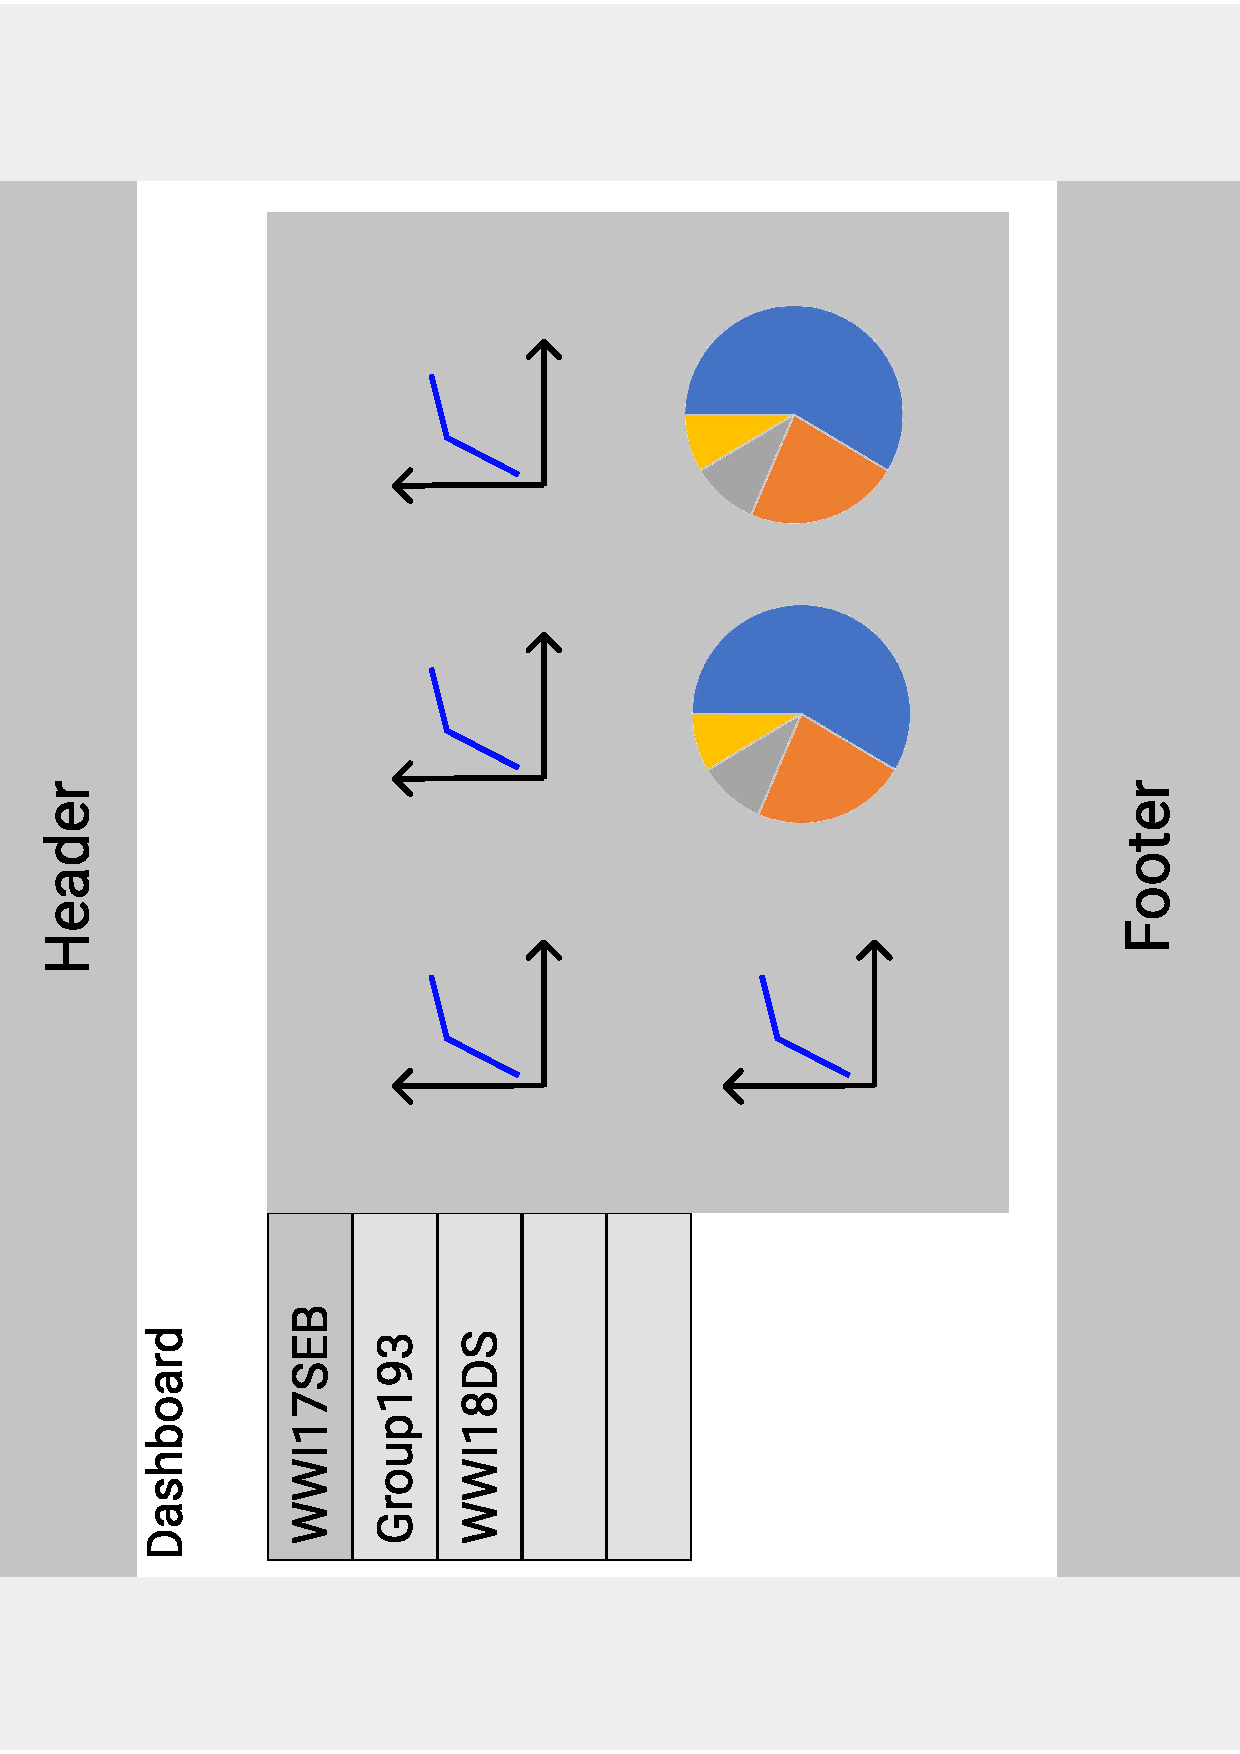
\includegraphics[width=0.7\textwidth]{img/konzeption/client/dashboard}
	\captionsetup{justification=centering, format=plain}
	\caption[Mock-Up des Dashboards]{Mock-Up des Dashboards \\\figma}
	\label{fig:MockDashboard}
\end{figure}

